% Options for packages loaded elsewhere
\PassOptionsToPackage{unicode}{hyperref}
\PassOptionsToPackage{hyphens}{url}
\PassOptionsToPackage{dvipsnames,svgnames,x11names}{xcolor}
%
\documentclass[
  letterpaper,
  DIV=11,
  numbers=noendperiod]{scrartcl}
\usepackage{amsmath,amssymb}
\usepackage{lmodern}
\usepackage{iftex}
\ifPDFTeX
  \usepackage[T1]{fontenc}
  \usepackage[utf8]{inputenc}
  \usepackage{textcomp} % provide euro and other symbols
\else % if luatex or xetex
  \usepackage{unicode-math}
  \defaultfontfeatures{Scale=MatchLowercase}
  \defaultfontfeatures[\rmfamily]{Ligatures=TeX,Scale=1}
\fi
% Use upquote if available, for straight quotes in verbatim environments
\IfFileExists{upquote.sty}{\usepackage{upquote}}{}
\IfFileExists{microtype.sty}{% use microtype if available
  \usepackage[]{microtype}
  \UseMicrotypeSet[protrusion]{basicmath} % disable protrusion for tt fonts
}{}
\makeatletter
\@ifundefined{KOMAClassName}{% if non-KOMA class
  \IfFileExists{parskip.sty}{%
    \usepackage{parskip}
  }{% else
    \setlength{\parindent}{0pt}
    \setlength{\parskip}{6pt plus 2pt minus 1pt}}
}{% if KOMA class
  \KOMAoptions{parskip=half}}
\makeatother
\usepackage{xcolor}
\IfFileExists{xurl.sty}{\usepackage{xurl}}{} % add URL line breaks if available
\IfFileExists{bookmark.sty}{\usepackage{bookmark}}{\usepackage{hyperref}}
\hypersetup{
  pdftitle={Data Visualization with Seaborn},
  pdfauthor={Alier Reng},
  colorlinks=true,
  linkcolor={blue},
  filecolor={Maroon},
  citecolor={Blue},
  urlcolor={Blue},
  pdfcreator={LaTeX via pandoc}}
\urlstyle{same} % disable monospaced font for URLs
\usepackage{color}
\usepackage{fancyvrb}
\newcommand{\VerbBar}{|}
\newcommand{\VERB}{\Verb[commandchars=\\\{\}]}
\DefineVerbatimEnvironment{Highlighting}{Verbatim}{commandchars=\\\{\}}
% Add ',fontsize=\small' for more characters per line
\usepackage{framed}
\definecolor{shadecolor}{RGB}{241,243,245}
\newenvironment{Shaded}{\begin{snugshade}}{\end{snugshade}}
\newcommand{\AlertTok}[1]{\textcolor[rgb]{0.68,0.00,0.00}{#1}}
\newcommand{\AnnotationTok}[1]{\textcolor[rgb]{0.37,0.37,0.37}{#1}}
\newcommand{\AttributeTok}[1]{\textcolor[rgb]{0.40,0.46,0.14}{#1}}
\newcommand{\BaseNTok}[1]{\textcolor[rgb]{0.68,0.00,0.00}{#1}}
\newcommand{\BuiltInTok}[1]{\textcolor[rgb]{0.00,0.46,0.62}{#1}}
\newcommand{\CharTok}[1]{\textcolor[rgb]{0.13,0.47,0.30}{#1}}
\newcommand{\CommentTok}[1]{\textcolor[rgb]{0.37,0.37,0.37}{#1}}
\newcommand{\CommentVarTok}[1]{\textcolor[rgb]{0.37,0.37,0.37}{\textit{#1}}}
\newcommand{\ConstantTok}[1]{\textcolor[rgb]{0.56,0.35,0.01}{#1}}
\newcommand{\ControlFlowTok}[1]{\textcolor[rgb]{0.00,0.46,0.62}{#1}}
\newcommand{\DataTypeTok}[1]{\textcolor[rgb]{0.68,0.00,0.00}{#1}}
\newcommand{\DecValTok}[1]{\textcolor[rgb]{0.68,0.00,0.00}{#1}}
\newcommand{\DocumentationTok}[1]{\textcolor[rgb]{0.37,0.37,0.37}{\textit{#1}}}
\newcommand{\ErrorTok}[1]{\textcolor[rgb]{0.68,0.00,0.00}{#1}}
\newcommand{\ExtensionTok}[1]{\textcolor[rgb]{0.00,0.46,0.62}{#1}}
\newcommand{\FloatTok}[1]{\textcolor[rgb]{0.68,0.00,0.00}{#1}}
\newcommand{\FunctionTok}[1]{\textcolor[rgb]{0.28,0.35,0.67}{#1}}
\newcommand{\ImportTok}[1]{\textcolor[rgb]{0.00,0.46,0.62}{#1}}
\newcommand{\InformationTok}[1]{\textcolor[rgb]{0.37,0.37,0.37}{#1}}
\newcommand{\KeywordTok}[1]{\textcolor[rgb]{0.00,0.46,0.62}{#1}}
\newcommand{\NormalTok}[1]{\textcolor[rgb]{0.00,0.46,0.62}{#1}}
\newcommand{\OperatorTok}[1]{\textcolor[rgb]{0.37,0.37,0.37}{#1}}
\newcommand{\OtherTok}[1]{\textcolor[rgb]{0.00,0.46,0.62}{#1}}
\newcommand{\PreprocessorTok}[1]{\textcolor[rgb]{0.68,0.00,0.00}{#1}}
\newcommand{\RegionMarkerTok}[1]{\textcolor[rgb]{0.00,0.46,0.62}{#1}}
\newcommand{\SpecialCharTok}[1]{\textcolor[rgb]{0.37,0.37,0.37}{#1}}
\newcommand{\SpecialStringTok}[1]{\textcolor[rgb]{0.13,0.47,0.30}{#1}}
\newcommand{\StringTok}[1]{\textcolor[rgb]{0.13,0.47,0.30}{#1}}
\newcommand{\VariableTok}[1]{\textcolor[rgb]{0.07,0.07,0.07}{#1}}
\newcommand{\VerbatimStringTok}[1]{\textcolor[rgb]{0.13,0.47,0.30}{#1}}
\newcommand{\WarningTok}[1]{\textcolor[rgb]{0.37,0.37,0.37}{\textit{#1}}}
\usepackage{longtable,booktabs,array}
\usepackage{calc} % for calculating minipage widths
% Correct order of tables after \paragraph or \subparagraph
\usepackage{etoolbox}
\makeatletter
\patchcmd\longtable{\par}{\if@noskipsec\mbox{}\fi\par}{}{}
\makeatother
% Allow footnotes in longtable head/foot
\IfFileExists{footnotehyper.sty}{\usepackage{footnotehyper}}{\usepackage{footnote}}
\makesavenoteenv{longtable}
\usepackage{graphicx}
\makeatletter
\def\maxwidth{\ifdim\Gin@nat@width>\linewidth\linewidth\else\Gin@nat@width\fi}
\def\maxheight{\ifdim\Gin@nat@height>\textheight\textheight\else\Gin@nat@height\fi}
\makeatother
% Scale images if necessary, so that they will not overflow the page
% margins by default, and it is still possible to overwrite the defaults
% using explicit options in \includegraphics[width, height, ...]{}
\setkeys{Gin}{width=\maxwidth,height=\maxheight,keepaspectratio}
% Set default figure placement to htbp
\makeatletter
\def\fps@figure{htbp}
\makeatother
\setlength{\emergencystretch}{3em} % prevent overfull lines
\providecommand{\tightlist}{%
  \setlength{\itemsep}{0pt}\setlength{\parskip}{0pt}}
\setcounter{secnumdepth}{-\maxdimen} % remove section numbering
\KOMAoption{captions}{tableheading}
\makeatletter
\makeatother
\makeatletter
\@ifpackageloaded{caption}{}{\usepackage{caption}}
\AtBeginDocument{%
\renewcommand*\contentsname{Table of contents}
\renewcommand*\listfigurename{List of Figures}
\renewcommand*\listtablename{List of Tables}
\renewcommand*\figurename{Figure}
\renewcommand*\tablename{Table}
}
\@ifpackageloaded{float}{}{\usepackage{float}}
\floatstyle{ruled}
\@ifundefined{c@chapter}{\newfloat{codelisting}{h}{lop}}{\newfloat{codelisting}{h}{lop}[chapter]}
\floatname{codelisting}{Listing}
\newcommand*\listoflistings{\listof{codelisting}{List of Listings}}
\makeatother
\makeatletter
\@ifpackageloaded{caption}{}{\usepackage{caption}}
\@ifpackageloaded{subcaption}{}{\usepackage{subcaption}}
\makeatother
\makeatletter
\makeatother
\ifLuaTeX
  \usepackage{selnolig}  % disable illegal ligatures
\fi

\title{Data Visualization with Seaborn}
\author{Alier Reng}
\date{April 23, 2022}

\begin{document}
\maketitle

\hypertarget{visualizing-the-tips-dataset-with-seaborn}{%
\subsection{Visualizing the tips Dataset with
Seaborn}\label{visualizing-the-tips-dataset-with-seaborn}}

This tutorial serves two purposes: 1) showcase \texttt{Quarto}, the next
generation of \texttt{RMarkdown}, and 2) illustrate how to visualize
data in \textbf{Python} with \texttt{seaborn}.

So, why \texttt{Quarto}?

According to its website, \emph{quarto.org}, \texttt{Quarto} \emph{``is
an open-source scientific and technical publishing system built on
\href{https://pandoc.org/}{Pandoc}.''}

\texttt{Quarto} enables data scientists and analysts to:

\begin{itemize}
\item
  Create dynamic content with
  \href{https://quarto.org/docs/computations/python.html}{Python},
  \href{https://quarto.org/docs/computations/r.html}{R},
  \href{https://quarto.org/docs/computations/julia.html}{Julia}, and
  \href{https://quarto.org/docs/computations/ojs.html}{Observable};
\item
  Author documents as plain text markdown or
  \href{https://jupyter.org/}{Jupyter} notebooks;
\item
  Publish high-quality articles, reports, presentations, websites,
  blogs, and books in HTML, PDF, MS Word, ePub, and more; and
\item
  Author with scientific markdown, including equations, citations,
  crossrefs, figure panels, callouts, advanced layout, and more.
  \textbf{\emph{(https://quarto.org/)}}
\end{itemize}

And why \texttt{seaborn}?

\texttt{Seaborn} is a \textbf{Python} data visualization library built
on top of \texttt{matplotlib}.

\begin{quote}
Seaborn is a Python data visualization library based on
\href{https://matplotlib.org/}{matplotlib}. It provides a high-level
interface for drawing attractive and informative statistical graphics.
\emph{(https://seaborn.pydata.org/)}
\end{quote}

Now let's get started.

\hypertarget{loading-the-libraries}{%
\subsubsection{Loading the Libraries}\label{loading-the-libraries}}

Here we will load \texttt{seaborn}, \texttt{matplotlib},
\texttt{pandas}, and \texttt{numpy}.

\begin{Shaded}
\begin{Highlighting}[]
\CommentTok{\# Import libraries}
\ImportTok{import}\NormalTok{ pandas }\ImportTok{as}\NormalTok{ pd}
\ImportTok{import}\NormalTok{ numpy }\ImportTok{as}\NormalTok{ np}
\CommentTok{\# Install and load the seaborn package}
\CommentTok{\#!pip install seaborn; the alias "sns" stands for Samuel Norman Seaborn from "The West Wing" television show}
\ImportTok{import}\NormalTok{ seaborn }\ImportTok{as}\NormalTok{ sns}
\ImportTok{import}\NormalTok{ matplotlib.pyplot }\ImportTok{as}\NormalTok{ plt}

\CommentTok{\# Initialize seaborn styling; context}
\NormalTok{sns.set\_style(}\StringTok{\textquotesingle{}white\textquotesingle{}}\NormalTok{)}
\NormalTok{sns.set\_context(}\StringTok{\textquotesingle{}notebook\textquotesingle{}}\NormalTok{)}
\end{Highlighting}
\end{Shaded}

\hypertarget{loading-the-dataset}{%
\subsubsection{Loading the Dataset}\label{loading-the-dataset}}

In this tutorial, we will use the \texttt{tips} dataset.

\begin{Shaded}
\begin{Highlighting}[]
\NormalTok{tips\_df }\OperatorTok{=}\NormalTok{ sns.load\_dataset(}\StringTok{\textquotesingle{}tips\textquotesingle{}}\NormalTok{)}
\end{Highlighting}
\end{Shaded}

\hypertarget{inspecting-the-data}{%
\subsubsection{Inspecting the data}\label{inspecting-the-data}}

\begin{Shaded}
\begin{Highlighting}[]
\CommentTok{\# Inspect the first 5 rows.}
\NormalTok{tips\_df.head()}
\end{Highlighting}
\end{Shaded}

\begin{tabular}{lrrllllr}
\toprule
{} &  total\_bill &   tip &     sex & smoker &  day &    time &  size \\
\midrule
0 &       16.99 &  1.01 &  Female &     No &  Sun &  Dinner &     2 \\
1 &       10.34 &  1.66 &    Male &     No &  Sun &  Dinner &     3 \\
2 &       21.01 &  3.50 &    Male &     No &  Sun &  Dinner &     3 \\
3 &       23.68 &  3.31 &    Male &     No &  Sun &  Dinner &     2 \\
4 &       24.59 &  3.61 &  Female &     No &  Sun &  Dinner &     4 \\
\bottomrule
\end{tabular}

\begin{Shaded}
\begin{Highlighting}[]
\CommentTok{\# Inspect the last 5 rows.}
\NormalTok{tips\_df.tail()}
\end{Highlighting}
\end{Shaded}

\begin{tabular}{lrrllllr}
\toprule
{} &  total\_bill &   tip &     sex & smoker &   day &    time &  size \\
\midrule
239 &       29.03 &  5.92 &    Male &     No &   Sat &  Dinner &     3 \\
240 &       27.18 &  2.00 &  Female &    Yes &   Sat &  Dinner &     2 \\
241 &       22.67 &  2.00 &    Male &    Yes &   Sat &  Dinner &     2 \\
242 &       17.82 &  1.75 &    Male &     No &   Sat &  Dinner &     2 \\
243 &       18.78 &  3.00 &  Female &     No &  Thur &  Dinner &     2 \\
\bottomrule
\end{tabular}

\hypertarget{checking-for-missing-values}{%
\subsubsection{Checking for Missing
Values}\label{checking-for-missing-values}}

\begin{Shaded}
\begin{Highlighting}[]
\CommentTok{\# Check if there are missing values.}
\NormalTok{tips\_df.isna().}\BuiltInTok{sum}\NormalTok{()}
\end{Highlighting}
\end{Shaded}

\begin{tabular}{lr}
\toprule
{} &  0 \\
\midrule
total\_bill &  0 \\
tip        &  0 \\
sex        &  0 \\
smoker     &  0 \\
day        &  0 \\
time       &  0 \\
size       &  0 \\
\bottomrule
\end{tabular}

There are no missing values.

\hypertarget{performing-a-quick-summary}{%
\subsubsection{Performing a Quick
Summary}\label{performing-a-quick-summary}}

\begin{Shaded}
\begin{Highlighting}[]
\CommentTok{\# Summarizing the data to get better understanding of our dataset; transpose the results for better view.}
\NormalTok{tips\_df.describe().T}
\end{Highlighting}
\end{Shaded}

\begin{tabular}{lrrrrrrrr}
\toprule
{} &  count &       mean &       std &   min &      25\% &     50\% &      75\% &    max \\
\midrule
total\_bill &  244.0 &  19.785943 &  8.902412 &  3.07 &  13.3475 &  17.795 &  24.1275 &  50.81 \\
tip        &  244.0 &   2.998279 &  1.383638 &  1.00 &   2.0000 &   2.900 &   3.5625 &  10.00 \\
size       &  244.0 &   2.569672 &  0.951100 &  1.00 &   2.0000 &   2.000 &   3.0000 &   6.00 \\
\bottomrule
\end{tabular}

\begin{Shaded}
\begin{Highlighting}[]
\CommentTok{\# Group by sex and smoker columns; compute the mean and round to 2 decimal places}

\CommentTok{\# Select desired columns.}
\NormalTok{cols }\OperatorTok{=}\NormalTok{ [}\StringTok{\textquotesingle{}sex\textquotesingle{}}\NormalTok{, }\StringTok{\textquotesingle{}smoker\textquotesingle{}}\NormalTok{, }\StringTok{\textquotesingle{}day\textquotesingle{}}\NormalTok{, }\StringTok{\textquotesingle{}total\_bill\textquotesingle{}}\NormalTok{, }\StringTok{\textquotesingle{}tip\textquotesingle{}}\NormalTok{]}

\NormalTok{df\_1 }\OperatorTok{=}\NormalTok{ (tips\_df}
\NormalTok{       [cols]}
\NormalTok{       .groupby([}\StringTok{\textquotesingle{}sex\textquotesingle{}}\NormalTok{, }\StringTok{\textquotesingle{}smoker\textquotesingle{}}\NormalTok{, }\StringTok{\textquotesingle{}day\textquotesingle{}}\NormalTok{])}
\NormalTok{       .mean()}
\NormalTok{       .}\BuiltInTok{round}\NormalTok{(}\DecValTok{2}\NormalTok{)}
\NormalTok{)}

\CommentTok{\# View the outputa}
\NormalTok{df\_1}
\end{Highlighting}
\end{Shaded}

\begin{tabular}{lllrr}
\toprule
       &    &     &  total\_bill &   tip \\
sex & smoker & day &             &       \\
\midrule
Male & Yes & Thur &       19.17 &  3.06 \\
       &    & Fri &       20.45 &  2.74 \\
       &    & Sat &       21.84 &  2.88 \\
       &    & Sun &       26.14 &  3.52 \\
       & No & Thur &       18.49 &  2.94 \\
       &    & Fri &       17.48 &  2.50 \\
       &    & Sat &       19.93 &  3.26 \\
       &    & Sun &       20.40 &  3.12 \\
Female & Yes & Thur &       19.22 &  2.99 \\
       &    & Fri &       12.65 &  2.68 \\
       &    & Sat &       20.27 &  2.87 \\
       &    & Sun &       16.54 &  3.50 \\
       & No & Thur &       16.01 &  2.46 \\
       &    & Fri &       19.37 &  3.12 \\
       &    & Sat &       19.00 &  2.72 \\
       &    & Sun &       20.82 &  3.33 \\
\bottomrule
\end{tabular}

\begin{Shaded}
\begin{Highlighting}[]
\CommentTok{\# Group by sex and smoker columns; compute the mean and round to 2 decimal places.}
\NormalTok{df\_2 }\OperatorTok{=}\NormalTok{ (tips\_df}
\NormalTok{        [cols]}
\NormalTok{        .groupby([}\StringTok{\textquotesingle{}sex\textquotesingle{}}\NormalTok{, }\StringTok{\textquotesingle{}smoker\textquotesingle{}}\NormalTok{])}
\NormalTok{        .mean()}
\NormalTok{        .}\BuiltInTok{round}\NormalTok{(}\DecValTok{2}\NormalTok{)}
\NormalTok{)}

\CommentTok{\# View the outputa}
\NormalTok{df\_2}
\end{Highlighting}
\end{Shaded}

\begin{tabular}{llrr}
\toprule
       &    &  total\_bill &   tip \\
sex & smoker &             &       \\
\midrule
Male & Yes &       22.28 &  3.05 \\
       & No &       19.79 &  3.11 \\
Female & Yes &       17.98 &  2.93 \\
       & No &       18.11 &  2.77 \\
\bottomrule
\end{tabular}

\begin{Shaded}
\begin{Highlighting}[]
\CommentTok{\# Group by the sex column; compute the mean and round to 2 decimal places}
\NormalTok{df\_3 }\OperatorTok{=}\NormalTok{ (tips\_df}
\NormalTok{        [cols]}
\NormalTok{        .groupby([}\StringTok{\textquotesingle{}sex\textquotesingle{}}\NormalTok{])}
\NormalTok{        .mean()}
\NormalTok{        .}\BuiltInTok{round}\NormalTok{(}\DecValTok{2}\NormalTok{)}
\NormalTok{)}

\CommentTok{\# View the outputa}
\NormalTok{df\_3}
\end{Highlighting}
\end{Shaded}

\begin{tabular}{lrr}
\toprule
{} &  total\_bill &   tip \\
sex    &             &       \\
\midrule
Male   &       20.74 &  3.09 \\
Female &       18.06 &  2.83 \\
\bottomrule
\end{tabular}

\hypertarget{visualizing-data-with-seaborn}{%
\subsubsection{\texorpdfstring{Visualizing Data with
\texttt{seaborn}}{Visualizing Data with seaborn}}\label{visualizing-data-with-seaborn}}

Let's begin with the \texttt{scatterplot}. However, we will use
\texttt{relplot} instead of \texttt{scatterplot} because the
\texttt{relplot} allows us to create subplots in a single figure.

\begin{Shaded}
\begin{Highlighting}[]
\CommentTok{\# Plot a scatterplot with the relplot() function}
\NormalTok{sc\_g }\OperatorTok{=}\NormalTok{ sns.relplot(x }\OperatorTok{=} \StringTok{\textquotesingle{}total\_bill\textquotesingle{}}\NormalTok{, }
\NormalTok{            y }\OperatorTok{=} \StringTok{\textquotesingle{}tip\textquotesingle{}}\NormalTok{,}
\NormalTok{            data }\OperatorTok{=}\NormalTok{ tips\_df,}
\NormalTok{            kind }\OperatorTok{=} \StringTok{\textquotesingle{}scatter\textquotesingle{}}\NormalTok{,}
\NormalTok{            hue }\OperatorTok{=} \StringTok{\textquotesingle{}smoker\textquotesingle{}}\NormalTok{,}
\NormalTok{            style }\OperatorTok{=} \StringTok{\textquotesingle{}smoker\textquotesingle{}}
\NormalTok{          )}
 
\CommentTok{\# Add the title}
\NormalTok{sc\_g.figure.suptitle(}\StringTok{\textquotesingle{}Tip vs Total Bill\textquotesingle{}}\NormalTok{)}
\NormalTok{sc\_g.}\BuiltInTok{set}\NormalTok{(xlabel }\OperatorTok{=} \StringTok{\textquotesingle{}Total Bill\textquotesingle{}}\NormalTok{,}
\NormalTok{         ylabel }\OperatorTok{=} \StringTok{\textquotesingle{}Tip\textquotesingle{}}\NormalTok{)}
         
\CommentTok{\# Show the plot.}
\NormalTok{plt.show()}
\end{Highlighting}
\end{Shaded}

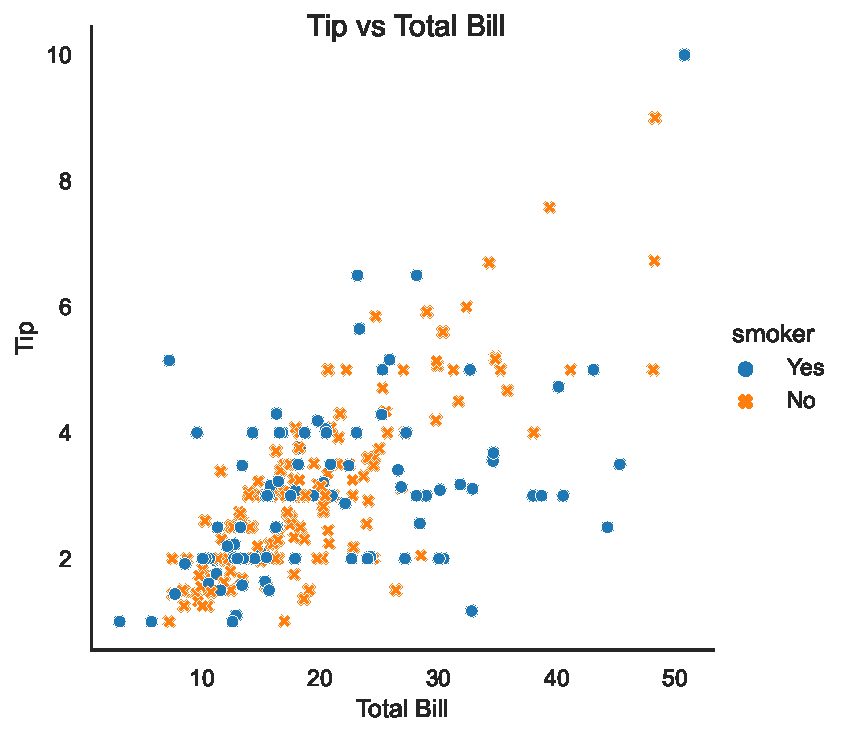
\includegraphics{data_visualization_with_seaborn_files/figure-pdf/cell-11-output-1.pdf}

\begin{Shaded}
\begin{Highlighting}[]
\CommentTok{\# Plot a scatterplot with the relplot() function}
\NormalTok{sc\_g }\OperatorTok{=}\NormalTok{ sns.relplot(x }\OperatorTok{=} \StringTok{\textquotesingle{}total\_bill\textquotesingle{}}\NormalTok{, }
\NormalTok{            y }\OperatorTok{=} \StringTok{\textquotesingle{}tip\textquotesingle{}}\NormalTok{,}
\NormalTok{            data }\OperatorTok{=}\NormalTok{ tips\_df,}
\NormalTok{            kind }\OperatorTok{=} \StringTok{\textquotesingle{}scatter\textquotesingle{}}\NormalTok{,}
\NormalTok{            hue }\OperatorTok{=} \StringTok{\textquotesingle{}smoker\textquotesingle{}}\NormalTok{,}
\NormalTok{            col }\OperatorTok{=} \StringTok{\textquotesingle{}time\textquotesingle{}}\NormalTok{,}
\NormalTok{            style }\OperatorTok{=} \StringTok{\textquotesingle{}smoker\textquotesingle{}}
\NormalTok{          )}
 
\CommentTok{\# Add the title}
\NormalTok{sc\_g.figure.suptitle(}\StringTok{\textquotesingle{}Tip vs Total Bill\textquotesingle{}}\NormalTok{)}
\NormalTok{sc\_g.}\BuiltInTok{set}\NormalTok{(xlabel }\OperatorTok{=} \StringTok{\textquotesingle{}Total Bill\textquotesingle{}}\NormalTok{,}
\NormalTok{         ylabel }\OperatorTok{=} \StringTok{\textquotesingle{}Tip\textquotesingle{}}\NormalTok{)}
         
\CommentTok{\# Show the plot.}
\NormalTok{plt.show()}
\end{Highlighting}
\end{Shaded}

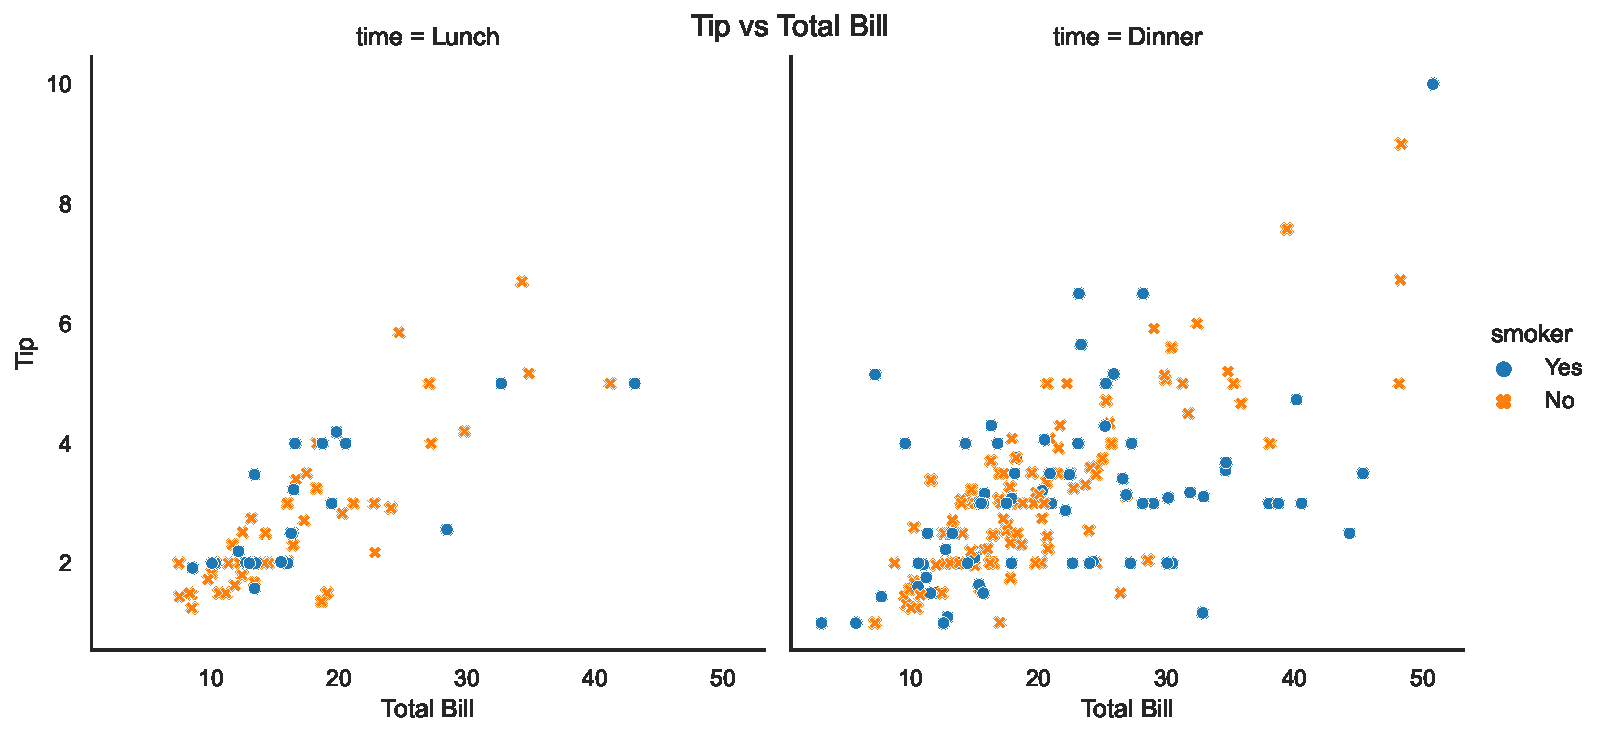
\includegraphics{data_visualization_with_seaborn_files/figure-pdf/cell-12-output-1.pdf}

\hypertarget{plotting-categorical-plots}{%
\subsubsection{Plotting Categorical
Plots}\label{plotting-categorical-plots}}

Here we will use the \texttt{catplot()} function because it enables us
to create subplots with \texttt{col=} and \texttt{row=} easily.

\begin{Shaded}
\begin{Highlighting}[]
\CommentTok{\# Plot the countplot.}
\NormalTok{count\_g }\OperatorTok{=}\NormalTok{ sns.catplot(}
\NormalTok{    x }\OperatorTok{=} \StringTok{\textquotesingle{}sex\textquotesingle{}}\NormalTok{,}
\NormalTok{    data }\OperatorTok{=}\NormalTok{ tips\_df,}
\NormalTok{    kind }\OperatorTok{=} \StringTok{\textquotesingle{}count\textquotesingle{}}
\NormalTok{)}

\NormalTok{count\_g.figure.suptitle(}\StringTok{\textquotesingle{}Countplot by Sex\textquotesingle{}}\NormalTok{)}
\NormalTok{plt.show()}
\end{Highlighting}
\end{Shaded}

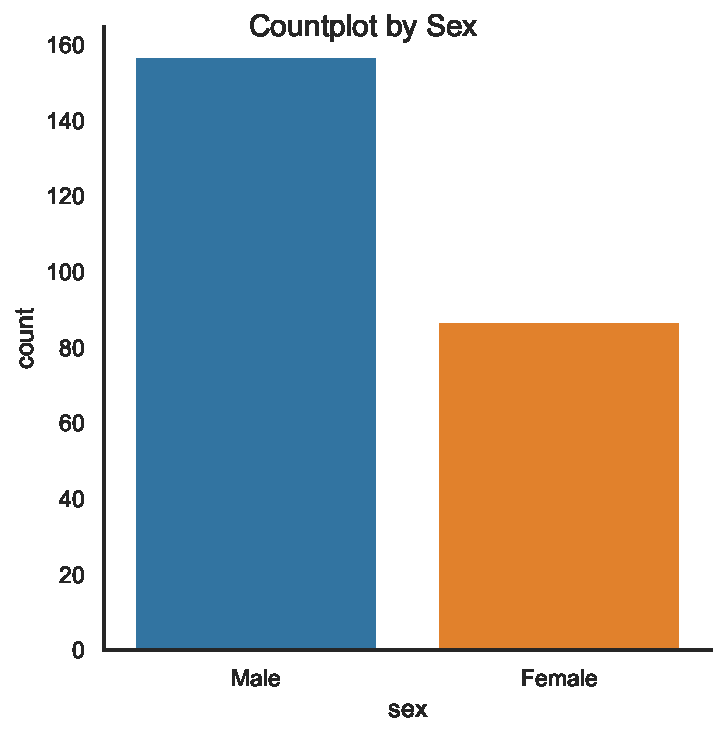
\includegraphics{data_visualization_with_seaborn_files/figure-pdf/cell-13-output-1.pdf}

\begin{Shaded}
\begin{Highlighting}[]
\CommentTok{\# Plot the countplot.}
\NormalTok{count\_g }\OperatorTok{=}\NormalTok{ sns.catplot(}
\NormalTok{    x }\OperatorTok{=} \StringTok{\textquotesingle{}smoker\textquotesingle{}}\NormalTok{,}
\NormalTok{    data }\OperatorTok{=}\NormalTok{ tips\_df,}
\NormalTok{    kind }\OperatorTok{=} \StringTok{\textquotesingle{}count\textquotesingle{}}\NormalTok{,}
\NormalTok{    hue }\OperatorTok{=} \StringTok{\textquotesingle{}sex\textquotesingle{}}
\NormalTok{)}

\NormalTok{count\_g.figure.suptitle(}\StringTok{\textquotesingle{}Countplot by Smoker\textquotesingle{}}\NormalTok{)}
\NormalTok{plt.show()}
\end{Highlighting}
\end{Shaded}

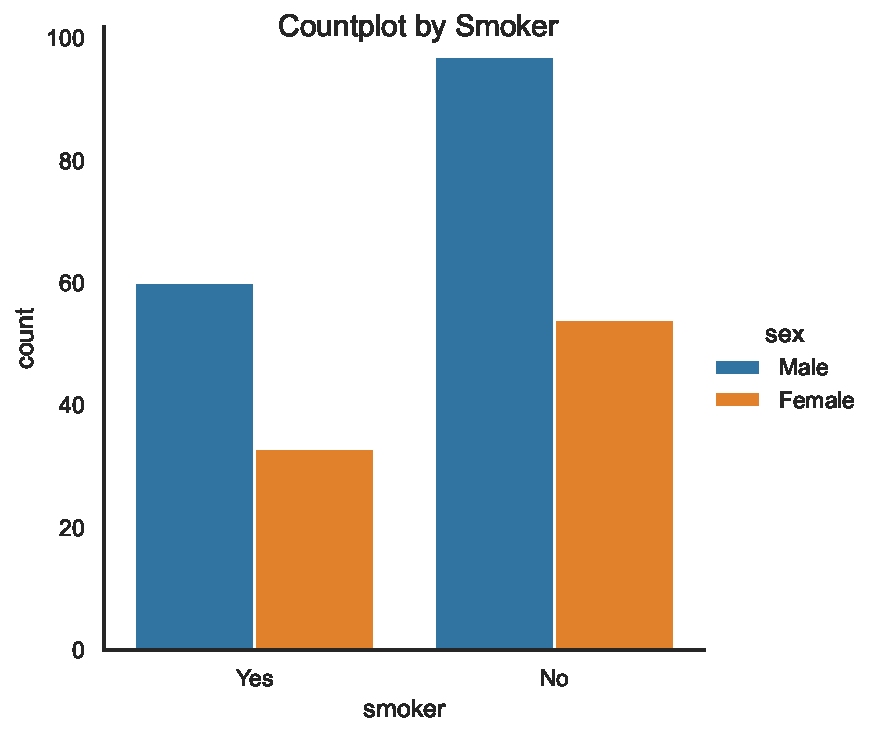
\includegraphics{data_visualization_with_seaborn_files/figure-pdf/cell-14-output-1.pdf}

\begin{Shaded}
\begin{Highlighting}[]
\NormalTok{bar\_g }\OperatorTok{=}\NormalTok{ sns.catplot(x }\OperatorTok{=} \StringTok{\textquotesingle{}day\textquotesingle{}}\NormalTok{,}
\NormalTok{                    y }\OperatorTok{=} \StringTok{\textquotesingle{}total\_bill\textquotesingle{}}\NormalTok{,}
\NormalTok{                    data }\OperatorTok{=}\NormalTok{ tips\_df,}
\NormalTok{                    kind }\OperatorTok{=} \StringTok{\textquotesingle{}bar\textquotesingle{}}
\NormalTok{                  )}
\CommentTok{\# Add the title}
\NormalTok{bar\_g.figure.suptitle(}\StringTok{\textquotesingle{}Total Bill by Days of the Week\textquotesingle{}}\NormalTok{)}
\NormalTok{bar\_g.}\BuiltInTok{set}\NormalTok{(xlabel }\OperatorTok{=} \StringTok{\textquotesingle{}Days of the Week\textquotesingle{}}\NormalTok{,}
\NormalTok{          ylabel }\OperatorTok{=} \StringTok{\textquotesingle{}Total Bill\textquotesingle{}}\NormalTok{)}

\NormalTok{plt.show()}
\end{Highlighting}
\end{Shaded}

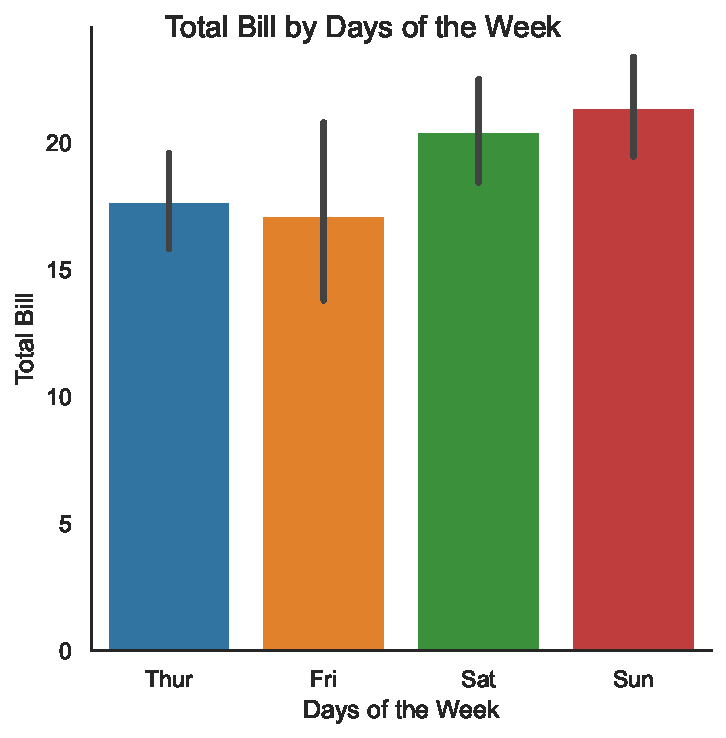
\includegraphics{data_visualization_with_seaborn_files/figure-pdf/cell-15-output-1.pdf}

\hypertarget{plotting-box-plots}{%
\subsubsection{Plotting Box Plots}\label{plotting-box-plots}}

A box plot shows the underlying distribution of quantitative data, and
it can quickly help us compare different data groups.

\begin{Shaded}
\begin{Highlighting}[]
\NormalTok{bp\_g }\OperatorTok{=}\NormalTok{ sns.catplot(x }\OperatorTok{=} \StringTok{\textquotesingle{}total\_bill\textquotesingle{}}\NormalTok{,}
\NormalTok{                   y }\OperatorTok{=} \StringTok{\textquotesingle{}time\textquotesingle{}}\NormalTok{,}
\NormalTok{                   data }\OperatorTok{=}\NormalTok{ tips\_df,}
\NormalTok{                   kind }\OperatorTok{=} \StringTok{\textquotesingle{}box\textquotesingle{}}\NormalTok{,}
\NormalTok{                   order }\OperatorTok{=}\NormalTok{ [}\StringTok{\textquotesingle{}Dinner\textquotesingle{}}\NormalTok{, }\StringTok{\textquotesingle{}Lunch\textquotesingle{}}\NormalTok{]}
\NormalTok{                  )}

\CommentTok{\# Add the title}
\NormalTok{bp\_g.figure.suptitle(}\StringTok{\textquotesingle{}Total Bill by Time of the Day\textquotesingle{}}\NormalTok{)}
\NormalTok{bp\_g.}\BuiltInTok{set}\NormalTok{(xlabel }\OperatorTok{=} \StringTok{\textquotesingle{}Total Bill\textquotesingle{}}\NormalTok{,}
\NormalTok{          ylabel }\OperatorTok{=} \StringTok{\textquotesingle{}Time of the Day\textquotesingle{}}\NormalTok{)}
          
\NormalTok{plt.show()}
\end{Highlighting}
\end{Shaded}

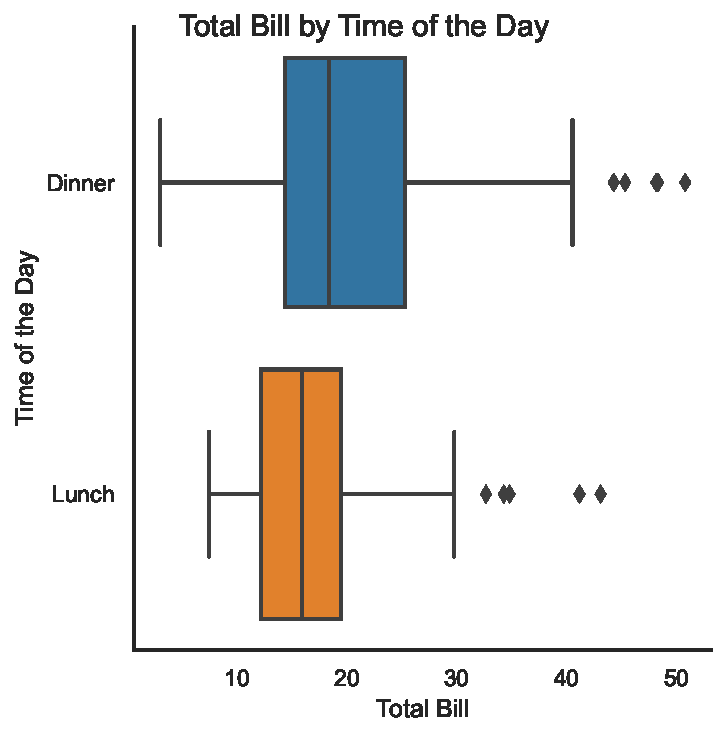
\includegraphics{data_visualization_with_seaborn_files/figure-pdf/cell-16-output-1.pdf}

\hypertarget{plotting-a-box-plot-without-outliers}{%
\subsubsection{Plotting a Box Plot without
Outliers}\label{plotting-a-box-plot-without-outliers}}

There're times when it may be necessary not to show outliers on a box
plot. If that's the case, we use \texttt{sym} to suppress them.

\begin{Shaded}
\begin{Highlighting}[]
\NormalTok{bp\_g }\OperatorTok{=}\NormalTok{ sns.catplot(x }\OperatorTok{=} \StringTok{\textquotesingle{}total\_bill\textquotesingle{}}\NormalTok{,}
\NormalTok{                   y }\OperatorTok{=} \StringTok{\textquotesingle{}time\textquotesingle{}}\NormalTok{,}
\NormalTok{                   data }\OperatorTok{=}\NormalTok{ tips\_df,}
\NormalTok{                   kind }\OperatorTok{=} \StringTok{\textquotesingle{}box\textquotesingle{}}\NormalTok{,}
\NormalTok{                   order }\OperatorTok{=}\NormalTok{ [}\StringTok{\textquotesingle{}Dinner\textquotesingle{}}\NormalTok{, }\StringTok{\textquotesingle{}Lunch\textquotesingle{}}\NormalTok{],}
\NormalTok{                   sym }\OperatorTok{=} \StringTok{\textquotesingle{}\textquotesingle{}}
\NormalTok{                  )}

\CommentTok{\# Formatting the plot}
\NormalTok{bp\_g.figure.suptitle(}\StringTok{\textquotesingle{}Total Bill by Time of the Day\textquotesingle{}}\NormalTok{)}
\NormalTok{bp\_g.}\BuiltInTok{set}\NormalTok{(xlabel }\OperatorTok{=} \StringTok{\textquotesingle{}Total Bill\textquotesingle{}}\NormalTok{,}
\NormalTok{          ylabel }\OperatorTok{=} \StringTok{\textquotesingle{}Time of the Day\textquotesingle{}}\NormalTok{)}
          
\CommentTok{\# Display the plot}
\NormalTok{plt.show()}
\end{Highlighting}
\end{Shaded}

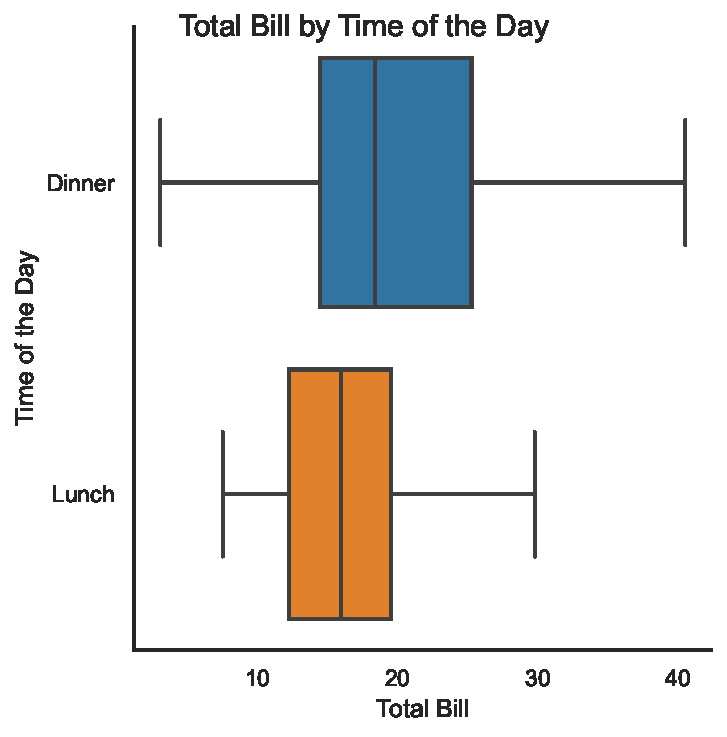
\includegraphics{data_visualization_with_seaborn_files/figure-pdf/cell-17-output-1.pdf}

\begin{Shaded}
\begin{Highlighting}[]
\CommentTok{\# Boxplot by smoker column.}
\NormalTok{b\_hue\_g }\OperatorTok{=}\NormalTok{ sns.catplot(x }\OperatorTok{=} \StringTok{\textquotesingle{}day\textquotesingle{}}\NormalTok{,}
\NormalTok{                      y }\OperatorTok{=} \StringTok{\textquotesingle{}total\_bill\textquotesingle{}}\NormalTok{,}
\NormalTok{                      data }\OperatorTok{=}\NormalTok{ tips\_df,}
\NormalTok{                      kind }\OperatorTok{=} \StringTok{\textquotesingle{}box\textquotesingle{}}\NormalTok{,}
\NormalTok{                      sym }\OperatorTok{=} \StringTok{\textquotesingle{}\textquotesingle{}}\NormalTok{,}
\NormalTok{                      hue }\OperatorTok{=} \StringTok{\textquotesingle{}smoker\textquotesingle{}}
\NormalTok{                  )}

\CommentTok{\# Formatting the plot}
\NormalTok{b\_hue\_g.figure.suptitle(}\StringTok{\textquotesingle{}Total Bill by Days of the Week\textquotesingle{}}\NormalTok{)}
\NormalTok{b\_hue\_g.}\BuiltInTok{set}\NormalTok{(xlabel }\OperatorTok{=} \StringTok{\textquotesingle{}Day of the Week\textquotesingle{}}\NormalTok{,}
\NormalTok{            ylabel }\OperatorTok{=} \StringTok{\textquotesingle{}Total Bill\textquotesingle{}}\NormalTok{)}
          
\CommentTok{\# Display the plot}
\NormalTok{plt.show()}
\end{Highlighting}
\end{Shaded}

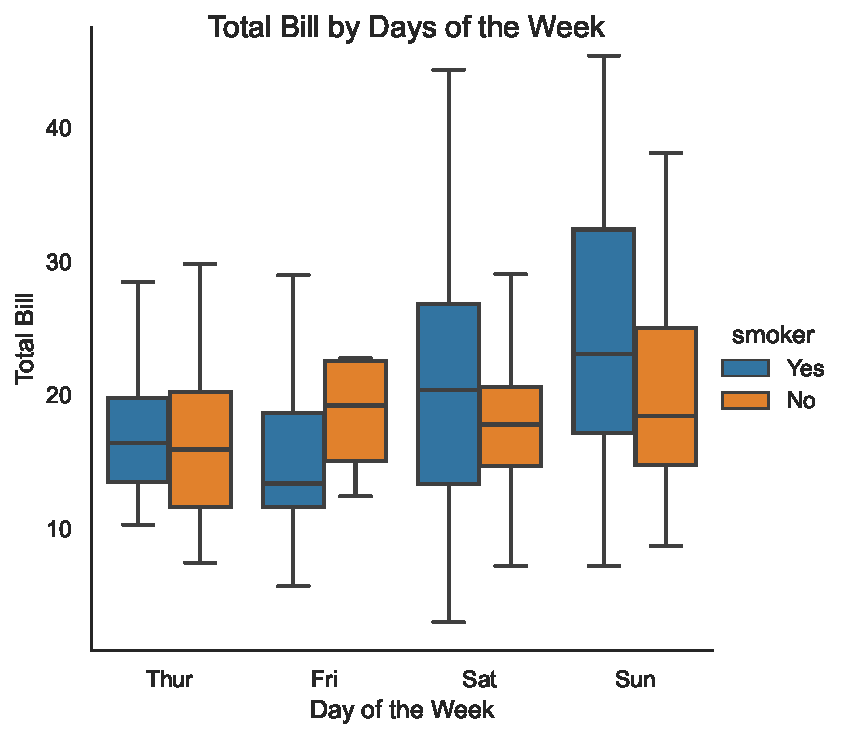
\includegraphics{data_visualization_with_seaborn_files/figure-pdf/cell-18-output-1.pdf}

\hypertarget{plotting-the-violin-plot}{%
\subsubsection{Plotting the Violin
Plot}\label{plotting-the-violin-plot}}

\begin{Shaded}
\begin{Highlighting}[]
\CommentTok{\# Plot a Violin Plot.}
\NormalTok{v\_g }\OperatorTok{=}\NormalTok{ sns.catplot(x }\OperatorTok{=} \StringTok{\textquotesingle{}day\textquotesingle{}}\NormalTok{,}
\NormalTok{                  y }\OperatorTok{=} \StringTok{\textquotesingle{}total\_bill\textquotesingle{}}\NormalTok{,}
\NormalTok{                  data }\OperatorTok{=}\NormalTok{ tips\_df,}
\NormalTok{                  kind }\OperatorTok{=} \StringTok{\textquotesingle{}violin\textquotesingle{}}\NormalTok{,}
\NormalTok{                  hue }\OperatorTok{=} \StringTok{\textquotesingle{}sex\textquotesingle{}}
\NormalTok{                )}
                    
\CommentTok{\# Formatting}
\NormalTok{v\_g.figure.suptitle(}\StringTok{"Total Bill by Days of the Week"}\NormalTok{)}
\NormalTok{v\_g.}\BuiltInTok{set}\NormalTok{(xlabel }\OperatorTok{=} \StringTok{\textquotesingle{}Days of the Week\textquotesingle{}}\NormalTok{,}
\NormalTok{        ylabel }\OperatorTok{=} \StringTok{\textquotesingle{}Total Bill\textquotesingle{}}\NormalTok{)}
  
\CommentTok{\# Display the plot      }
\NormalTok{plt.show()}
\end{Highlighting}
\end{Shaded}

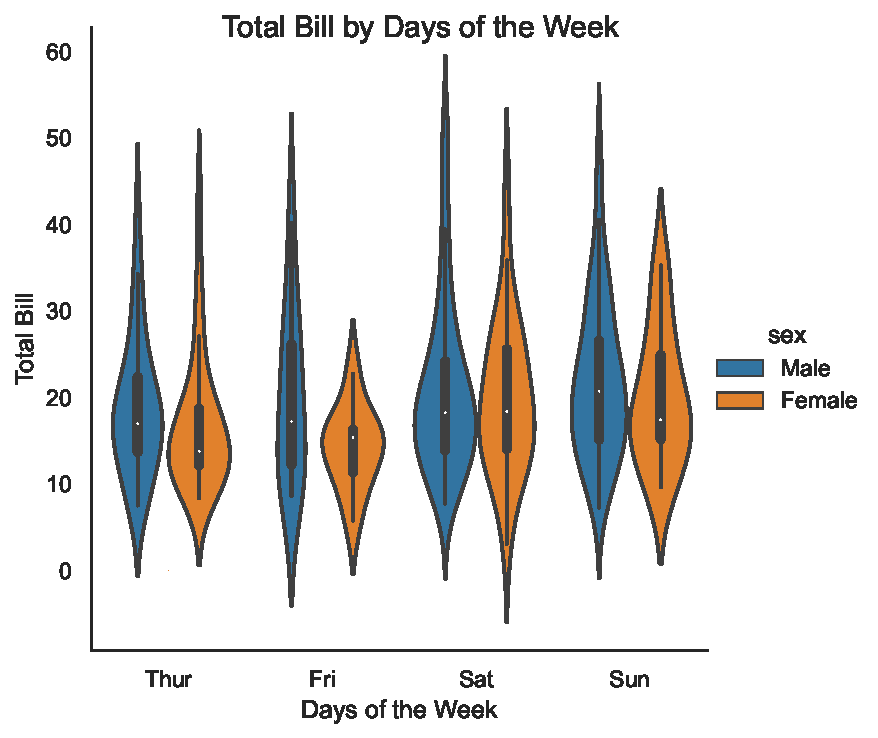
\includegraphics{data_visualization_with_seaborn_files/figure-pdf/cell-19-output-1.pdf}

\hypertarget{plotting-the-swarm-plot}{%
\subsubsection{Plotting the Swarm Plot}\label{plotting-the-swarm-plot}}

\begin{Shaded}
\begin{Highlighting}[]
\NormalTok{g }\OperatorTok{=}\NormalTok{ sns.catplot(x }\OperatorTok{=} \StringTok{\textquotesingle{}day\textquotesingle{}}\NormalTok{,}
\NormalTok{                y }\OperatorTok{=} \StringTok{\textquotesingle{}total\_bill\textquotesingle{}}\NormalTok{,}
\NormalTok{                data }\OperatorTok{=}\NormalTok{ tips\_df,}
\NormalTok{                kind }\OperatorTok{=} \StringTok{\textquotesingle{}violin\textquotesingle{}}\NormalTok{,}
\NormalTok{                inner }\OperatorTok{=} \VariableTok{None}
\NormalTok{                )}
                

\CommentTok{\# Plot a swarm plot}
\NormalTok{sns.swarmplot(x }\OperatorTok{=} \StringTok{\textquotesingle{}day\textquotesingle{}}\NormalTok{, }
\NormalTok{              y }\OperatorTok{=} \StringTok{\textquotesingle{}total\_bill\textquotesingle{}}\NormalTok{, }
\NormalTok{              color }\OperatorTok{=}\StringTok{"k"}\NormalTok{, }
\NormalTok{              size }\OperatorTok{=} \DecValTok{3}\NormalTok{, }
\NormalTok{              data }\OperatorTok{=}\NormalTok{ tips\_df,}
\NormalTok{              ax }\OperatorTok{=}\NormalTok{ g.ax}
\NormalTok{            )}
            
\CommentTok{\# Display the plot}
\NormalTok{plt.show()}
\end{Highlighting}
\end{Shaded}

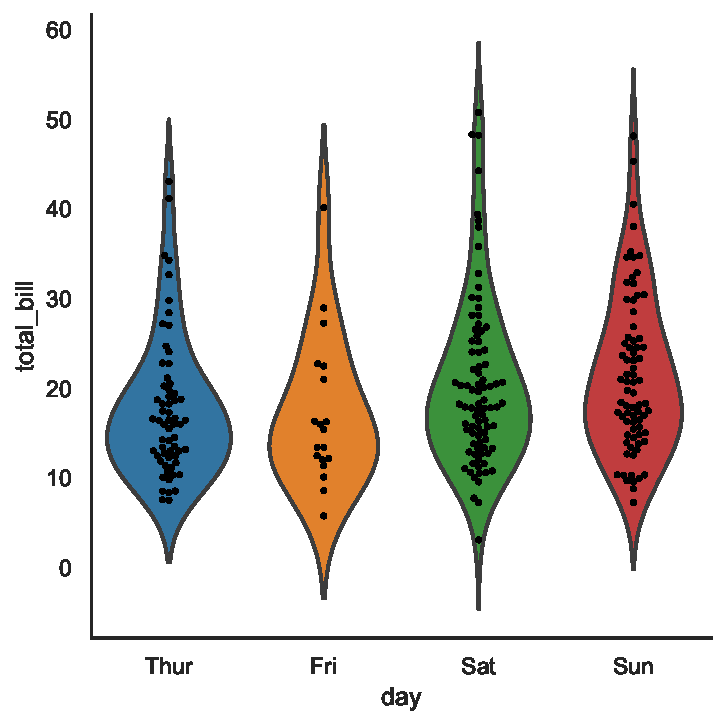
\includegraphics{data_visualization_with_seaborn_files/figure-pdf/cell-20-output-1.pdf}

\begin{Shaded}
\begin{Highlighting}[]
\CommentTok{\# Plot a swarm plot}
\NormalTok{sns.catplot(x }\OperatorTok{=} \StringTok{\textquotesingle{}day\textquotesingle{}}\NormalTok{, }
\NormalTok{            y }\OperatorTok{=} \StringTok{\textquotesingle{}total\_bill\textquotesingle{}}\NormalTok{, }
\NormalTok{            col }\OperatorTok{=} \StringTok{\textquotesingle{}time\textquotesingle{}}\NormalTok{, }
\NormalTok{            aspect }\OperatorTok{=} \FloatTok{.8}\NormalTok{, }
\NormalTok{            data }\OperatorTok{=}\NormalTok{ tips\_df,}
\NormalTok{            kind }\OperatorTok{=} \StringTok{\textquotesingle{}swarm\textquotesingle{}}\NormalTok{,}
\NormalTok{            hue }\OperatorTok{=} \StringTok{\textquotesingle{}smoker\textquotesingle{}}
\NormalTok{            )}
            
\CommentTok{\# Display the plot}
\NormalTok{plt.show()}
\end{Highlighting}
\end{Shaded}

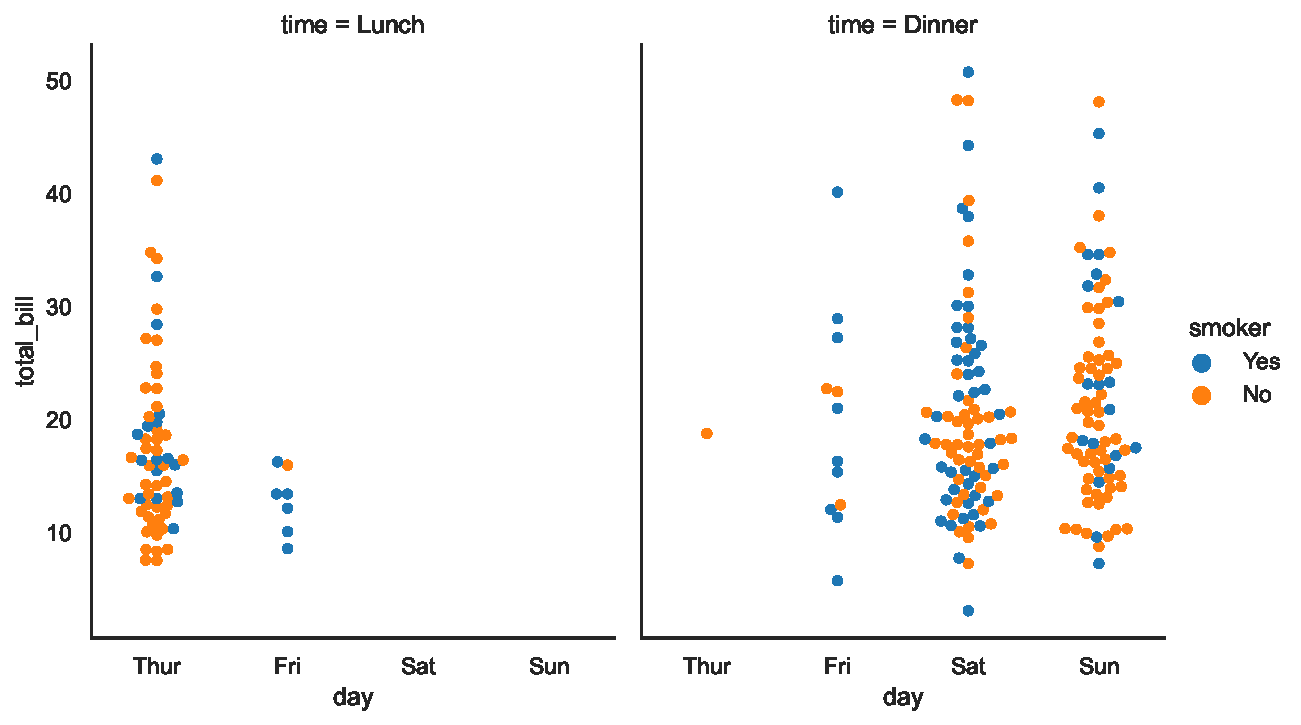
\includegraphics{data_visualization_with_seaborn_files/figure-pdf/cell-21-output-1.pdf}

\hypertarget{plotting-the-linear-regression-plot}{%
\subsubsection{Plotting the Linear Regression
Plot}\label{plotting-the-linear-regression-plot}}

\begin{Shaded}
\begin{Highlighting}[]
\CommentTok{\# Plot histogram}
\NormalTok{g }\OperatorTok{=}\NormalTok{ sns.lmplot(x }\OperatorTok{=} \StringTok{\textquotesingle{}total\_bill\textquotesingle{}}\NormalTok{, }
\NormalTok{               y }\OperatorTok{=} \StringTok{\textquotesingle{}tip\textquotesingle{}}\NormalTok{, }
\NormalTok{               hue }\OperatorTok{=} \StringTok{\textquotesingle{}smoker\textquotesingle{}}\NormalTok{,}
\NormalTok{               col }\OperatorTok{=} \StringTok{\textquotesingle{}time\textquotesingle{}}\NormalTok{,}
\NormalTok{               data }\OperatorTok{=}\NormalTok{ tips\_df,}
\NormalTok{               markers }\OperatorTok{=}\NormalTok{ [}\StringTok{\textquotesingle{}o\textquotesingle{}}\NormalTok{, }\StringTok{\textquotesingle{}*\textquotesingle{}}\NormalTok{], }
\NormalTok{               palette }\OperatorTok{=} \StringTok{\textquotesingle{}Set1\textquotesingle{}}\NormalTok{)}\OperatorTok{;}
\NormalTok{plt.show()}
\end{Highlighting}
\end{Shaded}

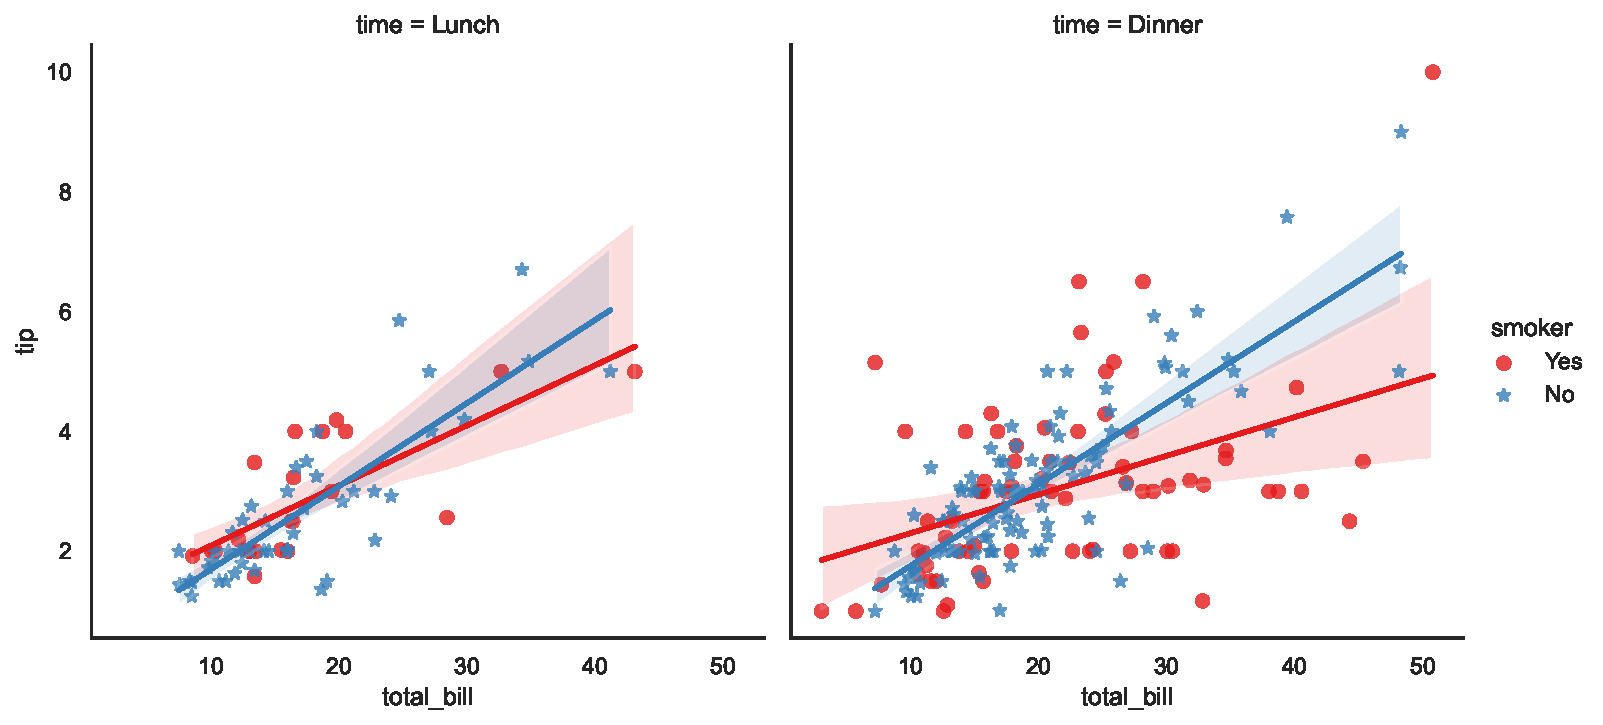
\includegraphics{data_visualization_with_seaborn_files/figure-pdf/cell-22-output-1.pdf}

\begin{Shaded}
\begin{Highlighting}[]
\NormalTok{sns.jointplot(x }\OperatorTok{=} \StringTok{\textquotesingle{}total\_bill\textquotesingle{}}\NormalTok{, }
\NormalTok{              y }\OperatorTok{=} \StringTok{\textquotesingle{}tip\textquotesingle{}}\NormalTok{, }
\NormalTok{              data }\OperatorTok{=}\NormalTok{ tips\_df, }
\NormalTok{              kind }\OperatorTok{=} \StringTok{\textquotesingle{}reg\textquotesingle{}}\NormalTok{)}\OperatorTok{;}
              
\CommentTok{\# Display the plot}
\NormalTok{plt.show()}
\end{Highlighting}
\end{Shaded}

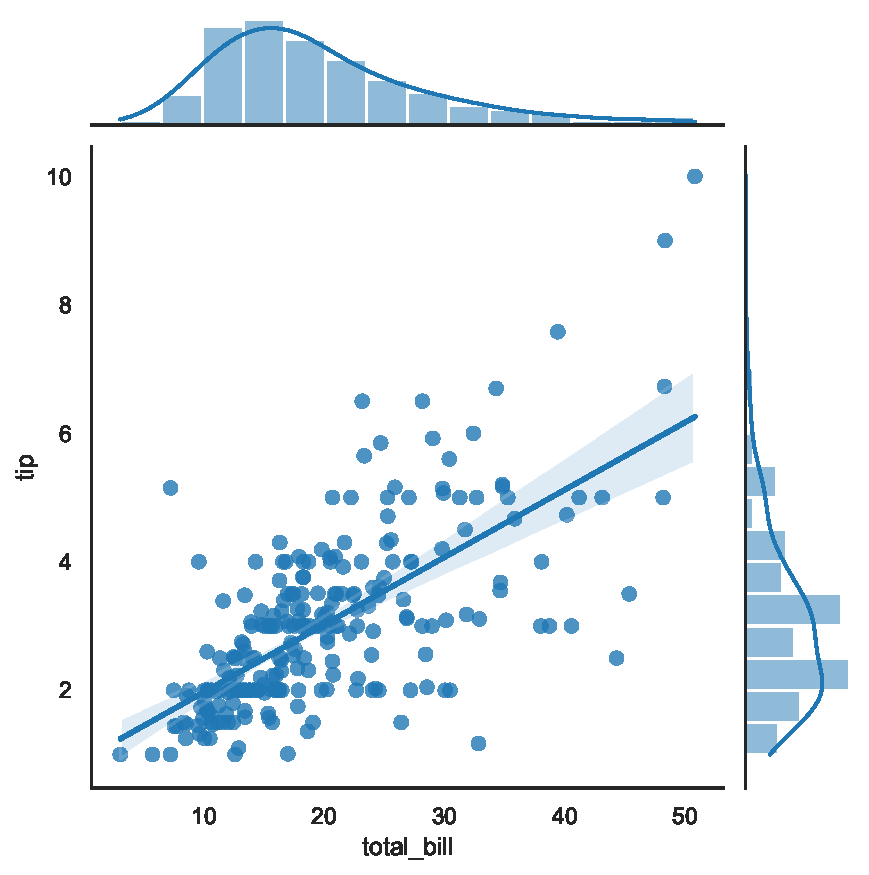
\includegraphics{data_visualization_with_seaborn_files/figure-pdf/cell-23-output-1.pdf}

\hypertarget{closing-remarks}{%
\subsubsection{Closing Remarks}\label{closing-remarks}}

This brief tutorial aims to teach users how to use Quarto to analyze
data with \texttt{Python} and visualize it with \texttt{seaborn}. A
thorough analysis would delve deep into describing the purposes of each
data visualization function. But for our purpose, we will leave things
as sketchy as they are.

\hypertarget{references}{%
\subsubsection{References}\label{references}}

\begin{itemize}
\item
  \href{https://seaborn.pydata.org/}{Seaborn library website}
\item
  \texttt{Datacamp\ course:} Introduction to
  \href{https://www.datacamp.com/courses/introduction-to-data-visualization-with-seaborn}{Introduction
  to Data Visualization with Seaborn}.
\end{itemize}

\end{document}
